\let\negmedspace\undefined
\let\negthickspace\undefined
\documentclass[journal]{IEEEtran}
\usepackage[a5paper, margin=10mm, onecolumn]{geometry}
%\usepackage{lmodern} % Ensure lmodern is loaded for pdflatex
\usepackage{tfrupee} % Include tfrupee package

\setlength{\headheight}{1cm} % Set the height of the header box
\setlength{\headsep}{0mm}     % Set the distance between the header box and the top of the text

\usepackage{gvv-book}
\usepackage{gvv}
\usepackage{cite}
\usepackage{amsmath,amssymb,amsfonts,amsthm}
\usepackage{algorithmic}
\usepackage{graphicx}
\usepackage{textcomp}
\usepackage{xcolor}
\usepackage{txfonts}
\usepackage{listings}
\usepackage{enumitem}
\usepackage{mathtools}
\usepackage{gensymb}
\usepackage{comment}
\usepackage[breaklinks=true]{hyperref}
\usepackage{tkz-euclide} 
\usepackage{listings}
\def\inputGnumericTable{}                                 
\usepackage[latin1]{inputenc}                                
\usepackage{color}                                            
\usepackage{array}                                            
\usepackage{longtable}                                       
\usepackage{calc}                                             
\usepackage{multirow}                                         
\usepackage{hhline}                                           
\usepackage{ifthen}                                           
\usepackage{lscape}
\begin{document}

\bibliographystyle{IEEEtran}
\vspace{3cm}

\title{9.3.3}
\author{AI25BTECH11012 - GARIGE UNNATHI}
% \maketitle
% \newpage
% \bigskip
{\let\newpage\relax\maketitle}


\renewcommand{\thefigure}{\theenumi}
\renewcommand{\thetable}{\theenumi}
\setlength{\intextsep}{10pt} % Space between text and floats


\numberwithin{equation}{enumi}
\numberwithin{figure}{enumi}
\renewcommand{\thetable}{\theenumi}


\textbf{Question}:\\
Find the area enclosed by the parabola 4y = 3$x^2$ and the line 2y = 3x + 12.\\

\textbf{Solution: }
The points of intersection of the line :

\begin{align}
  L : \vec{x} = \vec{h} + \kappa\vec{m}
\end{align}

with the conic  is given by 
\begin{align}
   \vec{x}_i = \vec{h} + \kappa_i\vec{m}
\end{align}

where :

\begin{align*}
 g(\vec{x}) = \vec{x}^{T}\vec{V}\vec{x} + 2\vec{u}^{T}\vec{x} + f\\ 
\kappa_i = \frac{1}
{\vec{m}^{T}\vec{V}\vec{m}}(-\vec{m}^{T}(\vec{V}\vec{h} + \vec{u}) \pm \sqrt{[\vec{m}^{T}(\vec{V}\vec{h}+\vec{u})]^{2} - g(\vec{h})(\vec{m}^{T}\vec{V}\vec{m})})
\end{align*}

For the parabola 3$x^2$ - 4y = 0
\begin{align}
   \vec{V} = \myvec{3 & 0\\0& 0}\\
   \vec{u} = \myvec{0\\-2}
\end{align}
For the line  2y = 3x + 12.
\begin{align}
  \vec{X} = \myvec{0\\6} + \kappa\myvec{0 \\ \frac{3}{2}}\\
  \vec{h} = \myvec{0\\6}\\
  \vec{m} = \myvec{0 \\ \frac{3}{2}}
\end{align}

Substituting and solving we get :
\begin{align}
 \kappa = \myvec{2 \\ -1}
\end{align}
so the points of intersection after solving using the equation 0.2 are :
\begin{align}
    \vec{X} = \myvec{4 \\ 12 } \quad and \quad \myvec{-2\\3}
\end{align}
Calculating the area  :
\begin{align}
    \int_{-2}^{4} \frac{3}{2}x + 6 - \frac{3}{4}x^2\,dx = 27 
\end{align}



\begin{figure}[h!]
   \centering
   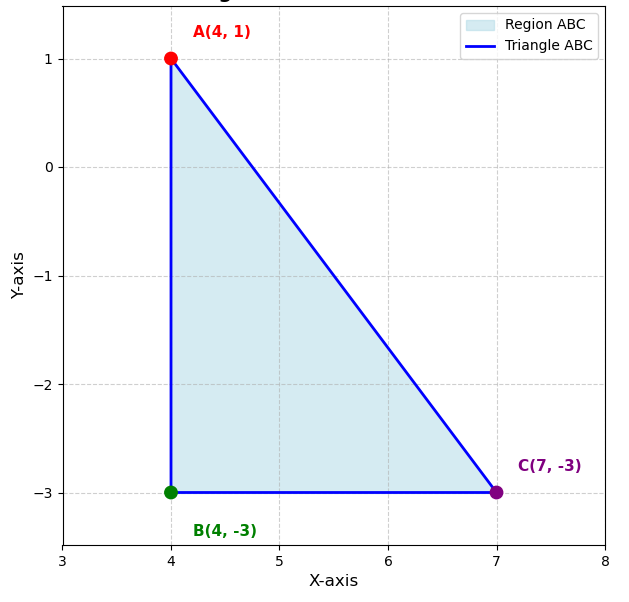
\includegraphics[width=0.7\linewidth]{/Users/unnathi/Documents/ee1030-2025/ai25btech11012/matgeo/9.3.3/figs/fig.png}
   \caption{}
   \label{stemplot}
\end{figure}





\end{document}
